%% ACM Double-Column Sample
%% Save this as "acm_ethernet.tex" (for example).
%% Compile with:  pdflatex acm_ethernet.tex   (twice)

\documentclass[sigconf]{acmart}

%% --- ACM Metadata / Copyright block: optional tweaks for preprint ---
\settopmatter{printacmref=false}    % Remove citation info below abstract
\renewcommand\footnotetextcopyrightpermission[1]{} % Remove footnote w/ conf info
\pagestyle{plain}                   % Remove running headers

%% --- Packages you likely need ---
\usepackage{amsmath,amssymb}
\usepackage{graphicx}
\usepackage{xcolor}
\usepackage{lipsum}     % for filler text
\usepackage{hyperref}

%% If you have multiple figures or want subfigures:
\usepackage{subfig}

%% If you do any fancy table layout, etc.:
\usepackage{booktabs}

%%%%%%%%%%%%%%%%%%%%%%%%%%%%%%%%%%%%%%%%%%%%%%%%%%%%%%%%%%%%%%%%%%%%%%%%
%% Title and author info
%%%%%%%%%%%%%%%%%%%%%%%%%%%%%%%%%%%%%%%%%%%%%%%%%%%%%%%%%%%%%%%%%%%%%%%%

\title{Ethernet: Distributed Packet Switching \\
       for Local Computer Networks}

\author{Robert M. Metcalfe}
\affiliation{%
  \institution{Xerox Palo Alto Research Center}
  \city{Palo Alto}
  \state{California}
  \country{USA}
}
\email{metcalfe@example.org}

\author{David R. Boggs}
\affiliation{%
  \institution{Xerox Palo Alto Research Center}
  \city{Palo Alto}
  \state{California}
  \country{USA}
}
\email{boggs@example.org}

%%%%%%%%%%%%%%%%%%%%%%%%%%%%%%%%%%%%%%%%%%%%%%%%%%%%%%%%%%%%%%%%%%%%%%%%
\begin{document}

\begin{abstract}
Ethernet is a branching broadcast communication system for carrying
digital data packets among locally distributed computing stations.
Design principles and implementation are described, based on experience
with an operating Ethernet of 100 nodes along a kilometer of coaxial cable.
A model for estimating performance under heavy loads and a packet protocol
for error-controlled communication are included for completeness.
\end{abstract}

\maketitle

%%%%%%%%%%%%%%%%%%%%%%%%%%%%%%%%%%%%%%%%%%%%%%%%%%%%%%%%%%%%%%%%%%%%%%%%
\section{Introduction}

One can characterize distributed computing as a spectrum of activities
varying in their degree of decentralization, with one extreme being remote
computer networking and the other extreme being multiprocessing.
\lipsum[1]

\begin{figure}[t]
  \centering
  % If your PDF figures exist in a subfolder "Figures", reference them accordingly:
  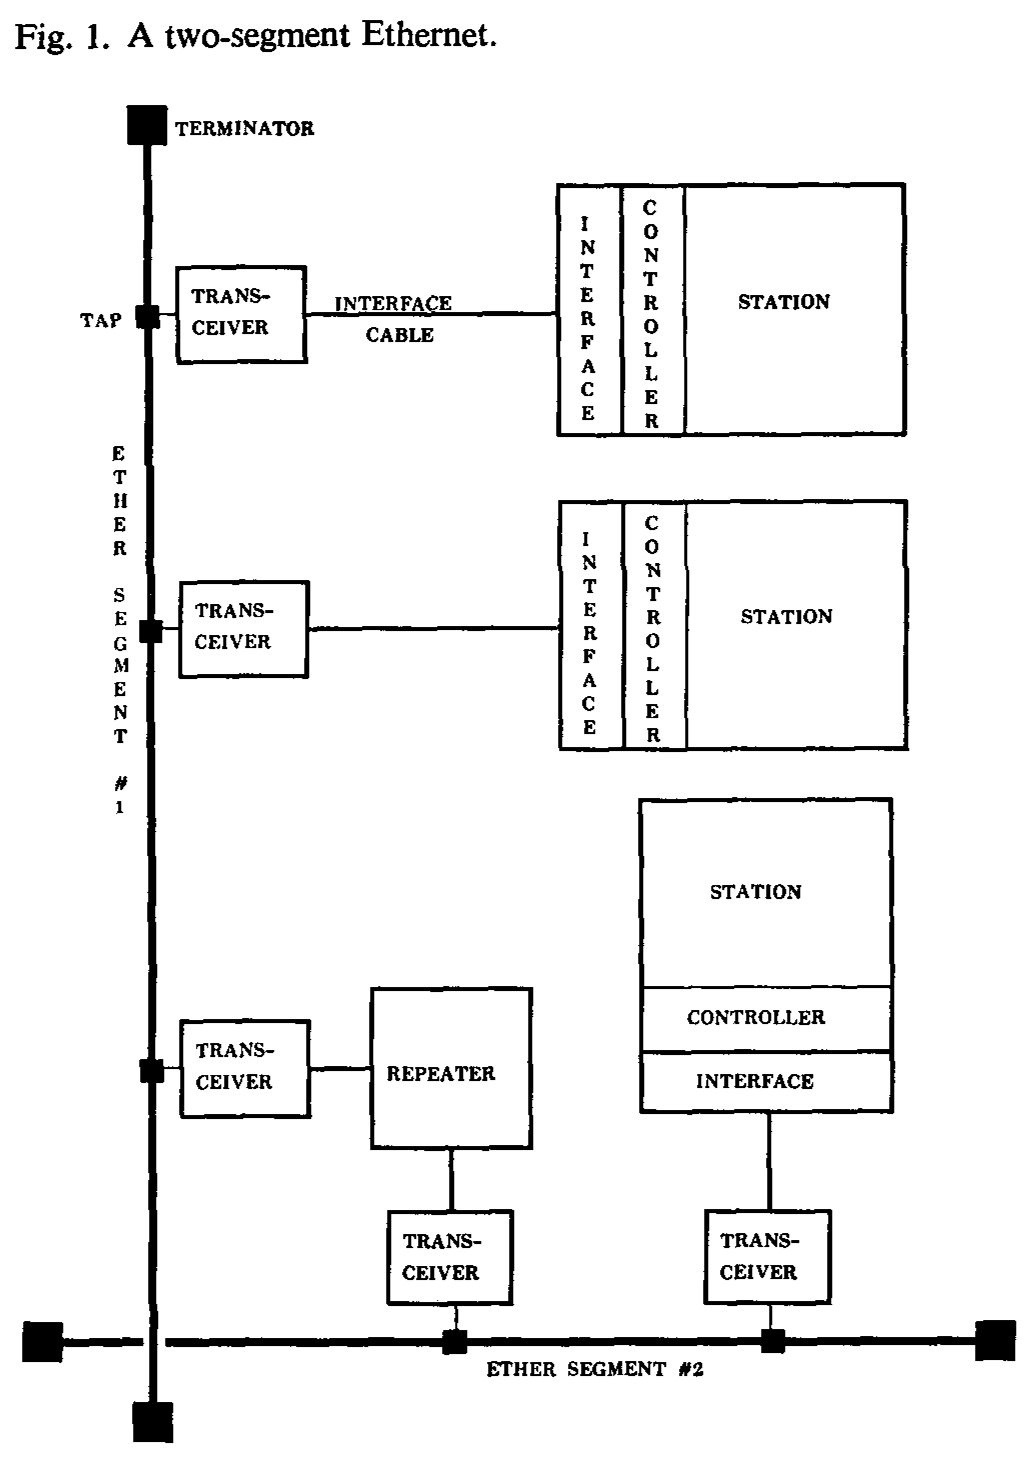
\includegraphics[width=\linewidth]{Figures/Ethernet-Fig-1.pdf}
  \caption{Ethernet Figure 1 (example).}
  \label{fig:eth1}
\end{figure}

\lipsum[2]

%%%%%%%%%%%%%%%%%%%%%%%%%%%%%%%%%%%%%%%%%%%%%%%%%%%%%%%%%%%%%%%%%%%%%%%%
\section{Background}

\subsection{Remote Computer Networking}
Computer networking evolved from telecommunications
terminal-computer communication, where the object was
to connect remote terminals to a central computing facility.
\lipsum[3]

\subsection{Multiprocessing}
Multiprocessing first took the form of connecting an
I/O controller to a large central computer; IBM’s ASP is a classic
example~\cite{Barnes1968}.
\lipsum[4]

%%%%%%%%%%%%%%%%%%%%%%%%%%%%%%%%%%%%%%%%%%%%%%%%%%%%%%%%%%%%%%%%%%%%%%%%
\section{Design Principles}

Our object is to design a communication system that can grow smoothly
to accommodate several buildings full of personal computers.
\lipsum[2]

\begin{figure}[t]
  \centering
  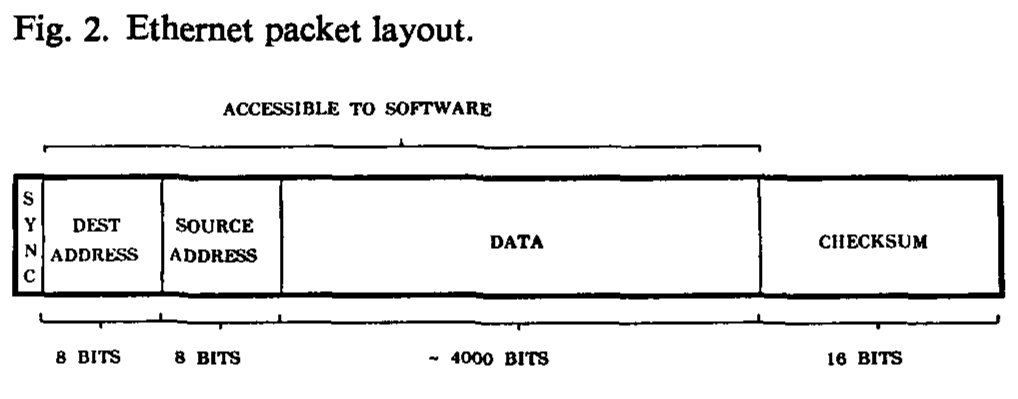
\includegraphics[width=0.8\linewidth]{Figures/Ethernet-Fig-2.pdf}
  \caption{Ethernet Figure 2.}
  \label{fig:eth2}
\end{figure}

\lipsum[2]

%%%%%%%%%%%%%%%%%%%%%%%%%%%%%%%%%%%%%%%%%%%%%%%%%%%%%%%%%%%%%%%%%%%%%%%%
\section{Implementation}

Our choices of 1\,km, 3\,Mbps, and 256 stations for the parameters of an
experimental Ethernet were based on characteristics of the locally distributed
environment and our assessments of what would be marginally achievable.
\lipsum[2]

%%%%%%%%%%%%%%%%%%%%%%%%%%%%%%%%%%%%%%%%%%%%%%%%%%%%%%%%%%%%%%%%%%%%%%%%
\section{Conclusion}

Our experience with an operating Ethernet leads us to conclude that emphasis
on distributed control was well placed. By keeping the shared components
to a minimum and passive, we have achieved a very high level of reliability.
\lipsum[2]

%%%%%%%%%%%%%%%%%%%%%%%%%%%%%%%%%%%%%%%%%%%%%%%%%%%%%%%%%%%%%%%%%%%%%%%%
\begin{acks}
We thank our colleagues at the Xerox Palo Alto Research Center,
especially Tat C.\ Lam, Butler W.\ Lampson, John F.\ Shoch, and
Charles P.\ Thacker, for their many contributions to the evolution
of Ethernet.
\end{acks}

%%%%%%%%%%%%%%%%%%%%%%%%%%%%%%%%%%%%%%%%%%%%%%%%%%%%%%%%%%%%%%%%%%%%%%%%
%% References: using thebibliography for short example
%% (For real ACM publications, you'd typically do:
%%   \bibliographystyle{ACM-Reference-Format}
%%   \bibliography{yourbibfile}
%%)

\begin{thebibliography}{99}

\bibitem{Barnes1968}
G.~H. Barnes, R.~M. Brown, M.~Kato, D.~J. Kuck, D.~L. Slotaick,
  and R.~A. Stokes.
\newblock The Illiac IV computer.
\newblock {\em IEEE Transactions on Computers}, C-17(8):758--770, 1968.

\bibitem{Metcalfe1976Ethernet}
R.~M. Metcalfe and D.~R. Boggs.
\newblock Ethernet: Distributed packet switching for local computer networks.
\newblock {\em Communications of the ACM}, 19(7):395--404, 1976.

\end{thebibliography}

\end{document}
